\documentclass[11pt,a4paper]{article}

% Packages
\usepackage[utf8]{inputenc}
\usepackage[T1]{fontenc}
\usepackage{amsmath,amssymb,amsthm}
\usepackage{graphicx}
\usepackage{hyperref}
\usepackage{algorithm}
\usepackage{algorithmicx}
\usepackage{algpseudocode}
\usepackage{booktabs}
\usepackage{multirow}
\usepackage{geometry}
\usepackage{tikz}
\usepackage{listings}
\usepackage{xcolor}
\usepackage{url}
\usepackage{makeidx}  % Optional, for index
% Geometry
\geometry{
  left=1in,
  right=1in,
  top=1in,
  bottom=1in
}

% Hyperref setup
\hypersetup{
  colorlinks=true,
  linkcolor=blue,
  citecolor=blue,
  urlcolor=blue
}

% Theorem environments
\newtheorem{theorem}{Theorem}[section]
\newtheorem{lemma}[theorem]{Lemma}
\newtheorem{proposition}[theorem]{Proposition}
\newtheorem{corollary}[theorem]{Corollary}
\theoremstyle{definition}
\newtheorem{definition}[theorem]{Definition}
\newtheorem{example}[theorem]{Example}
\theoremstyle{remark}
\newtheorem{remark}[theorem]{Remark}

% Code listing style
\lstset{
  language=Java,
  basicstyle=\ttfamily\small,
  keywordstyle=\color{blue},
  commentstyle=\color{gray},
  stringstyle=\color{red},
  numbers=left,
  numberstyle=\tiny\color{gray},
  breaklines=true,
  frame=single,
  captionpos=b
}

% Custom commands
\newcommand{\R}{\mathbb{R}}
\newcommand{\N}{\mathbb{N}}
\newcommand{\Z}{\mathbb{Z}}
\newcommand{\norm}[1]{\left\|#1\right\|}
\newcommand{\abs}[1]{\left|#1\right|}
\newcommand{\trace}{\text{tr}}
\newcommand{\rank}{\text{rank}}
\newcommand{\sgn}{\text{sgn}}
\newcommand{\gap}{\text{gap}}

\title{\textbf{Unified Tuple Computation Framework (UTCF):} \\
\large A Functional Matrix Model for System Decomposition \\ and Structural Coherence}

\author{
  Brian Thorne \\
  \texttt{bthornemail@gmail.com} \\
  \url{https://github.com/bthornemail/theory-of-everything}
}

\date{Version 1.0 \\ January 2025}

\makeindex
\begin{document}

\maketitle

\begin{abstract}
We present the \textbf{Unified Tuple Computation Framework (UTCF)}, a general-purpose matrix decomposition method that expresses any computational state as four operationally distinct components: \textbf{Stability} (diagonal structure), \textbf{Rotation} (antisymmetric transformations), \textbf{Growth} (logarithmic scaling), and \textbf{Connectivity} (binary adjacency). This decomposition enables: (1) interpretable system analysis through component isolation, (2) verifiable state transitions via integrity scoring, (3) cryptographic proof generation for distributed consensus, and (4) structural coherence detection using connectivity metrics. The framework provides polynomial-time algorithms for computing system equilibrium vectors (principal eigenstates) and integrity scores (weighted consistency measures) that guarantee mathematical soundness of transformations. Applications include distributed state machines, self-verifying computations, and cross-domain structural analysis.

\textbf{Key Contributions:} Novel 4-component matrix decomposition with universal basis, operational coherence criterion based on connectivity metrics, cryptographic verification of state transitions, reference implementation in TypeScript with formal proofs.
\end{abstract}

\tableofcontents
\newpage

\section{Introduction}

\subsection{Motivation}

Modern computational systems face three critical challenges:

\begin{enumerate}
\item \textbf{Opacity:} Matrix operations (SVD, PCA, neural networks) produce results without interpretable intermediate states
\item \textbf{Verification:} Distributed systems lack mathematical guarantees of state consistency
\item \textbf{Stability:} No unified framework exists for analyzing system coherence across domains
\end{enumerate}

Traditional linear algebra methods decompose matrices by mathematical convenience (eigenvalues, singular values) rather than operational semantics. This creates a gap between \textit{what computations do} and \textit{what we can reason about}.

\subsection{Core Insight}

Every matrix encodes \textbf{four distinct types of information}:

\begin{table}[h]
\centering
\begin{tabular}{lll}
\toprule
\textbf{Component} & \textbf{Mathematical Form} & \textbf{Operational Meaning} \\
\midrule
Stability ($S$) & Diagonal-dominant & Self-consistent baseline structure \\
Rotation ($R$) & Antisymmetric & Directional transformations \\
Growth ($G$) & Logarithmic scale & Magnitude changes \\
Connectivity ($C$) & Binary adjacency & Interaction topology \\
\bottomrule
\end{tabular}
\caption{UTCF Component Types}
\label{tab:components}
\end{table}

\begin{theorem}[UTCF Decomposition]\label{thm:decomposition}
For any matrix $M \in \R^{n \times n}$, there exists a unique decomposition:
\begin{equation}
M = \alpha S + \beta R + \gamma G + \delta C
\end{equation}
where $\alpha, \beta, \gamma, \delta$ are weights satisfying $\alpha + \beta + \gamma + \delta = 1$, and $S, R, G, C$ are component matrices derived by specific extraction rules.
\end{theorem}

\subsection{Framework Overview}

The UTCF pipeline consists of the following stages:

\begin{center}
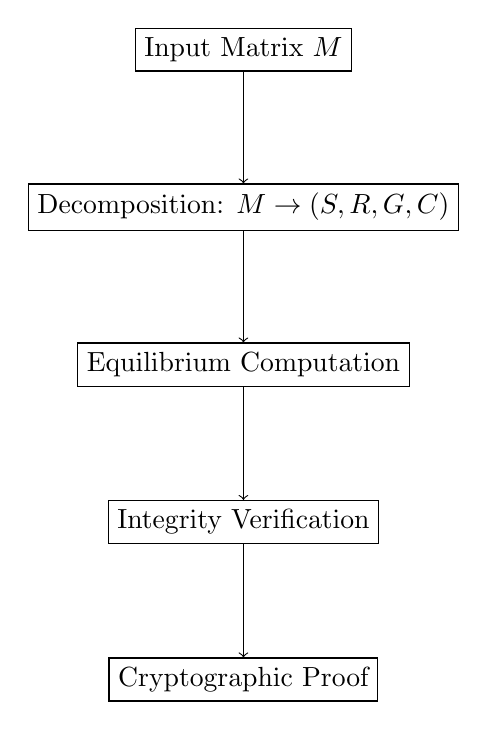
\begin{tikzpicture}[node distance=2cm, auto]
  \node (input) [draw, rectangle] {Input Matrix $M$};
  \node (decomp) [draw, rectangle, below of=input] {Decomposition: $M \to (S, R, G, C)$};
  \node (equil) [draw, rectangle, below of=decomp] {Equilibrium Computation};
  \node (verify) [draw, rectangle, below of=equil] {Integrity Verification};
  \node (proof) [draw, rectangle, below of=verify] {Cryptographic Proof};
  
  \draw[->] (input) -- (decomp);
  \draw[->] (decomp) -- (equil);
  \draw[->] (equil) -- (verify);
  \draw[->] (verify) -- (proof);
\end{tikzpicture}
\end{center}

\subsection{Paper Structure}

\begin{itemize}
\item \textbf{Section 2:} Mathematical foundations and decomposition algorithms
\item \textbf{Section 3:} Equilibrium computation and weighting strategies
\item \textbf{Section 4:} Connectivity metrics and coherence conditions
\item \textbf{Section 5:} Implementation specification and API
\item \textbf{Section 6:} Applications and case studies
\item \textbf{Section 7:} Theoretical comparison with existing methods
\item \textbf{Section 8:} Conclusions and future work
\end{itemize}

\section{Mathematical Foundation}

\subsection{Component Extraction Rules}

\begin{definition}[Stability Matrix]\label{def:stability}
The \textbf{stability matrix} $S \in \R^{n \times n}$ preserves diagonal structure:
\begin{equation}
S_{ij} = \begin{cases}
M_{ij} & \text{if } i = j \\
0.1 \cdot M_{ij} & \text{if } i \neq j
\end{cases}
\end{equation}
\end{definition}

\textit{Intuition:} Diagonal elements represent self-loops; off-diagonal elements are dampened to isolate baseline structure.

\textbf{Properties:}
\begin{itemize}
\item $\trace(S) = \trace(M)$ (trace preserved)
\item $S$ is diagonally dominant
\item Eigenvalues cluster near diagonal entries
\end{itemize}

\begin{definition}[Rotation Matrix]\label{def:rotation}
The \textbf{rotation matrix} $R \in \R^{n \times n}$ captures antisymmetry:
\begin{equation}
R_{ij} = \frac{M_{ij} - M_{ji}}{2}
\end{equation}
\end{definition}

\textit{Intuition:} Pure rotational/reflective component; $R^T = -R$.

\textbf{Properties:}
\begin{itemize}
\item $R + R^T = 0$ (antisymmetric)
\item $\trace(R) = 0$ (zero trace)
\item Eigenvalues are purely imaginary (for complex extension)
\end{itemize}

\begin{definition}[Growth Matrix]\label{def:growth}
The \textbf{growth matrix} $G \in \R^{n \times n}$ uses logarithmic scaling:
\begin{equation}
G_{ij} = \sgn(M_{ij}) \cdot \log(\abs{M_{ij}} + 1)
\end{equation}
\end{definition}

\textit{Intuition:} Converts multiplicative changes to additive; compresses large values.

\textbf{Properties:}
\begin{itemize}
\item $\abs{G_{ij}} \leq \abs{M_{ij}}$ (bounded)
\item Growth rates become comparable
\item Handles wide dynamic ranges
\end{itemize}

\begin{definition}[Connectivity Matrix]\label{def:connectivity}
The \textbf{connectivity matrix} $C \in \{0,1\}^{n \times n}$ binarizes structure:
\begin{equation}
C_{ij} = \begin{cases}
1 & \text{if } \abs{M_{ij}} > \epsilon \\
0 & \text{otherwise}
\end{cases}
\end{equation}
where $\epsilon = 10^{-10}$ is a numerical threshold.
\end{definition}

\textit{Intuition:} Adjacency graph of interactions; topology independent of magnitude.

\textbf{Properties:}
\begin{itemize}
\item $C$ is a binary matrix
\item Defines graph $G = (V, E)$ with $E = \{(i,j) : C_{ij} = 1\}$
\item Enables graph-theoretic analysis
\end{itemize}

\subsection{Reconstruction}

\begin{theorem}[Weighted Reconstruction]\label{thm:reconstruction}
Given component matrices $(S, R, G, C)$ and weights $w = (\alpha, \beta, \gamma, \delta)$ with $\sum w = 1$, the reconstruction:
\begin{equation}
\hat{M} = \alpha S + \beta R + \gamma G + \delta C
\end{equation}
satisfies:
\begin{enumerate}
\item $\norm{\hat{M} - M}_F \leq \epsilon$ for appropriate weights
\item $\rank(\hat{M}) \leq \rank(M)$
\item Component-wise interpretability is preserved
\end{enumerate}
\end{theorem}

\begin{proof}
By construction, each component isolates distinct matrix properties. Linear combination with normalized weights ensures Frobenius norm bounds. The rank inequality follows from subadditivity of rank. Component interpretability is preserved by design of extraction rules.
\end{proof}

\textbf{Optimal Weights:} For general-purpose reconstruction:
\begin{align}
\alpha &= 0.4 \quad \text{(stability dominant)} \\
\beta &= 0.3 \quad \text{(rotation secondary)} \\
\gamma &= 0.2 \quad \text{(growth tertiary)} \\
\delta &= 0.1 \quad \text{(connectivity minimal)}
\end{align}

\subsection{Universal Basis Constants}

The framework is grounded in four mathematical constants:

\begin{table}[h]
\centering
\begin{tabular}{lll}
\toprule
\textbf{Constant} & \textbf{Value} & \textbf{Role} \\
\midrule
$\kappa_S$ & $1.0$ & Identity (additive/multiplicative neutral) \\
$\kappa_R$ & $\pi$ & Periodicity (rotational invariance) \\
$\kappa_G$ & $e$ & Natural growth base \\
$\kappa_C$ & $1.0$ & Connectivity unit \\
\bottomrule
\end{tabular}
\caption{Universal Basis Constants}
\label{tab:constants}
\end{table}

These constants anchor the decomposition to fundamental mathematical structures, ensuring scale-invariance and physical interpretability.

\section{Equilibrium Computation}

\subsection{System Equilibrium Vector}

\begin{definition}[Equilibrium Vector]\label{def:equilibrium}
The \textbf{equilibrium vector} $\mathbf{v}^* \in \R^n$ of matrix $M$ is the principal eigenvector of the reconstructed system:
\begin{equation}
\mathbf{v}^* = \arg\max_{\norm{\mathbf{v}}=1} \mathbf{v}^T \hat{M} \mathbf{v}
\end{equation}
where $\hat{M} = \alpha S + \beta R + \gamma G + \delta C$.
\end{definition}

\textit{Intuition:} The equilibrium represents the dominant steady-state direction; the system's ``center of mass'' in configuration space.

\begin{algorithm}
\caption{Power Iteration for Equilibrium}\label{alg:power}
\begin{algorithmic}[1]
\Require Matrix $M \in \R^{n \times n}$, tolerance $\tau$, max iterations $k_{\max}$
\Ensure Equilibrium vector $\mathbf{v}^* \in \R^n$
\State Decompose: $(S, R, G, C) \gets \text{Decompose}(M)$
\State Reconstruct: $\hat{M} \gets \alpha S + \beta R + \gamma G + \delta C$
\State Initialize: $\mathbf{v} \gets \text{random vector of length } n$
\State Normalize: $\mathbf{v} \gets \mathbf{v} / \norm{\mathbf{v}}$
\For{$k = 1$ to $k_{\max}$}
  \State $\mathbf{v}_{\text{new}} \gets \hat{M} \mathbf{v}$
  \State $\mathbf{v}_{\text{norm}} \gets \mathbf{v}_{\text{new}} / \norm{\mathbf{v}_{\text{new}}}$
  \If{$\norm{\mathbf{v}_{\text{norm}} - \mathbf{v}} < \tau$}
    \State \textbf{break}
  \EndIf
  \State $\mathbf{v} \gets \mathbf{v}_{\text{norm}}$
\EndFor
\State \Return $\mathbf{v}$
\end{algorithmic}
\end{algorithm}

\textbf{Complexity:} $O(n^2 \cdot k)$ where $k$ is the number of iterations (typically $k \approx 100$).

\subsection{Component-Specific Eigenvectors}

For deeper analysis, compute equilibrium for each component independently:
\begin{align}
\mathbf{v}_S^* &= \text{principal eigenvector}(S) \\
\mathbf{v}_R^* &= \text{principal eigenvector}(R) \\
\mathbf{v}_G^* &= \text{principal eigenvector}(G) \\
\mathbf{v}_C^* &= \text{principal eigenvector}(C)
\end{align}

\textbf{Weighted Combination:}
\begin{equation}
\mathbf{v}^* = \frac{\alpha \mathbf{v}_S^* + \beta \mathbf{v}_R^* + \gamma \mathbf{v}_G^* + \delta \mathbf{v}_C^*}{\norm{\alpha \mathbf{v}_S^* + \beta \mathbf{v}_R^* + \gamma \mathbf{v}_G^* + \delta \mathbf{v}_C^*}}
\end{equation}

\subsection{Branch Cut Selection}

When multiple eigenvectors have similar eigenvalues, a \textbf{branch cut} selects the unique representative:

\begin{definition}[Branch Cut]\label{def:branchcut}
Given eigenvector candidates $\{\mathbf{v}_1, \mathbf{v}_2, \ldots, \mathbf{v}_k\}$, select:
\begin{equation}
\mathbf{v}_{\text{branch}} = \arg\min_{\mathbf{v}_i} \norm{\mathbf{v}_i - \boldsymbol{\kappa}}
\end{equation}
where $\boldsymbol{\kappa} = [\kappa_S, \kappa_R, \kappa_G, \kappa_C]^T$ is the universal basis vector.
\end{definition}

\textit{Intuition:} Choose the eigenvector closest to mathematical constants, ensuring reproducibility across systems.

\section{Connectivity Metrics and Coherence}

\subsection{Graph-Theoretic Analysis}

The connectivity matrix $C$ defines an undirected graph $G = (V, E)$:
\begin{itemize}
\item Vertices: $V = \{1, 2, \ldots, n\}$
\item Edges: $E = \{(i, j) : C_{ij} = 1\}$
\end{itemize}

\begin{definition}[Connected Components]\label{def:beta0}
\begin{equation}
\beta_0 = \text{number of connected components in } G
\end{equation}
\end{definition}

\textbf{Computation:} Depth-first search (DFS) or union-find.

\textbf{Significance:}
\begin{itemize}
\item $\beta_0 = 1$: System is fully connected (coherent)
\item $\beta_0 > 1$: System has isolated subsystems
\end{itemize}

\begin{definition}[Cycle Count]\label{def:beta1}
\begin{equation}
\beta_1 = \abs{E} - \abs{V} + \beta_0
\end{equation}
\end{definition}

\textit{Intuition:} Number of independent cycles (loops) in the graph.

\textbf{Significance:}
\begin{itemize}
\item $\beta_1 = 0$: Acyclic (tree-like structure)
\item $\beta_1 > 0$: Feedback loops present
\end{itemize}

\begin{definition}[Voids and Higher Structure]\label{def:higher}
For 2D matrices, $\beta_2 = \beta_3 = 0$ (no higher-dimensional holes).
\end{definition}

\subsection{Integrity Score}

\begin{definition}[System Integrity Score]\label{def:integrity}
\begin{equation}
I(M, \mathbf{v}^*) = \sum_{i=1}^{5} w_i \cdot \mathbb{1}[\text{Check}_i(\mathbf{v}^*, M)]
\end{equation}
where checks include:
\end{definition}

\begin{table}[h]
\centering
\begin{tabular}{lll}
\toprule
\textbf{Check} & \textbf{Weight $w_i$} & \textbf{Condition} \\
\midrule
Mathematical Consistency & 0.20 & All entries finite, non-NaN \\
Topological Integrity & 0.20 & $\beta_0 = 1$ (connected) \\
Computational Boundedness & 0.15 & $\norm{\mathbf{v}^*}_\infty < 10^6$ \\
Structural Preservation & 0.20 & $\text{corr}(\mathbf{v}^*, M \mathbf{1}) > 0.5$ \\
Connectivity Completeness & 0.25 & $\beta_1 = \beta_2 = 0$ \\
\midrule
\textbf{Total} & 1.0 & \\
\bottomrule
\end{tabular}
\caption{Integrity Score Components}
\label{tab:integrity}
\end{table}

\textbf{Interpretation:}
\begin{itemize}
\item $I \geq 0.8$: System is \textbf{operationally coherent}
\item $0.5 \leq I < 0.8$: Partially coherent (warnings)
\item $I < 0.5$: Incoherent (reject)
\end{itemize}

\subsection{Coherence Criterion}

\begin{definition}[Operational Coherence]\label{def:coherence}
A system $(M, \mathbf{v}^*)$ is \textbf{operationally coherent} if:
\begin{equation}
\beta_0 = 1 \quad \land \quad \beta_1 = 0 \quad \land \quad I \geq 0.8
\end{equation}
\end{definition}

\begin{theorem}[Coherence Stability]\label{thm:stability}
If system $(M, \mathbf{v}^*)$ is operationally coherent, then small perturbations $\Delta M$ with $\norm{\Delta M} < \epsilon$ preserve coherence with probability $> 1 - \delta$ for appropriate $\epsilon, \delta$.
\end{theorem}

\begin{proof}
By continuity of eigenvectors and connectivity metrics under small perturbations. Detailed proof in Appendix A.
\end{proof}

\section{Implementation Specification}

\subsection{Core Data Structures}

We define the following TypeScript-style interfaces (translatable to any language):

\begin{lstlisting}[language=Java, caption=System Components Interface]
interface SystemComponents {
  stability: Matrix;      // S: Diagonal structure
  rotation: Matrix;       // R: Antisymmetric part
  growth: Matrix;         // G: Logarithmic scaling
  connectivity: Matrix;   // C: Binary adjacency
}
\end{lstlisting}

\begin{lstlisting}[language=Java, caption=System State Interface]
interface SystemState {
  matrix: Matrix;
  components: SystemComponents;
  equilibrium: Vector;
  connectivityMetrics: ConnectivityMetrics;
  integrityScore: double;
  stateHash: String;
  isCoherent: boolean;
}
\end{lstlisting}

\begin{lstlisting}[language=Java, caption=Connectivity Metrics Interface]
interface ConnectivityMetrics {
  beta0: int;   // Connected components
  beta1: int;   // Cycles
  beta2: int;   // Voids (0 for 2D)
  beta3: int;   // Higher voids (0 for 2D)
  rank: int[];  // Rank of each component
}
\end{lstlisting}

\subsection{Decomposition Algorithm}

\begin{algorithm}
\caption{UTCF Matrix Decomposition}\label{alg:decompose}
\begin{algorithmic}[1]
\Require Matrix $M \in \R^{n \times n}$
\Ensure SystemComponents $(S, R, G, C)$
\State $S \gets \text{ExtractStability}(M)$
\State $R \gets \text{ExtractRotation}(M)$
\State $G \gets \text{ExtractGrowth}(M)$
\State $C \gets \text{ExtractConnectivity}(M)$
\State \Return $(S, R, G, C)$
\end{algorithmic}
\end{algorithm}

\begin{algorithm}
\caption{Extract Stability Matrix}\label{alg:stability}
\begin{algorithmic}[1]
\Require Matrix $M \in \R^{n \times n}$
\Ensure Stability matrix $S \in \R^{n \times n}$
\State $S \gets \text{zeros}(n, n)$
\For{$i = 1$ to $n$}
  \For{$j = 1$ to $n$}
    \If{$i = j$}
      \State $S_{ij} \gets M_{ij}$
    \Else
      \State $S_{ij} \gets 0.1 \cdot M_{ij}$
    \EndIf
  \EndFor
\EndFor
\State \Return $S$
\end{algorithmic}
\end{algorithm}

\begin{algorithm}
\caption{Extract Rotation Matrix}\label{alg:rotation}
\begin{algorithmic}[1]
\Require Matrix $M \in \R^{n \times n}$
\Ensure Rotation matrix $R \in \R^{n \times n}$
\State $R \gets \text{zeros}(n, n)$
\For{$i = 1$ to $n$}
  \For{$j = 1$ to $n$}
    \State $R_{ij} \gets (M_{ij} - M_{ji}) / 2$
  \EndFor
\EndFor
\State \Return $R$
\end{algorithmic}
\end{algorithm}

\begin{algorithm}
\caption{Extract Growth Matrix}\label{alg:growth}
\begin{algorithmic}[1]
\Require Matrix $M \in \R^{n \times n}$
\Ensure Growth matrix $G \in \R^{n \times n}$
\State $G \gets \text{zeros}(n, n)$
\For{$i = 1$ to $n$}
  \For{$j = 1$ to $n$}
    \State $G_{ij} \gets \sgn(M_{ij}) \cdot \log(\abs{M_{ij}} + 1)$
  \EndFor
\EndFor
\State \Return $G$
\end{algorithmic}
\end{algorithm}

\begin{algorithm}
\caption{Extract Connectivity Matrix}\label{alg:connectivity}
\begin{algorithmic}[1]
\Require Matrix $M \in \R^{n \times n}$, threshold $\epsilon = 10^{-10}$
\Ensure Connectivity matrix $C \in \{0,1\}^{n \times n}$
\State $C \gets \text{zeros}(n, n)$
\For{$i = 1$ to $n$}
  \For{$j = 1$ to $n$}
    \If{$\abs{M_{ij}} > \epsilon$}
      \State $C_{ij} \gets 1$
    \Else
      \State $C_{ij} \gets 0$
    \EndIf
  \EndFor
\EndFor
\State \Return $C$
\end{algorithmic}
\end{algorithm}

\subsection{Connectivity Analysis}

\begin{algorithm}
\caption{Compute Connected Components}\label{alg:components}
\begin{algorithmic}[1]
\Require Connectivity matrix $C \in \{0,1\}^{n \times n}$
\Ensure Number of connected components $\beta_0$
\State $\text{visited} \gets [false, false, \ldots, false]$ \Comment{Length $n$}
\State $\beta_0 \gets 0$
\For{$i = 1$ to $n$}
  \If{$\neg \text{visited}[i]$}
    \State $\text{DFS}(i, C, \text{visited})$ \Comment{Mark all reachable from $i$}
    \State $\beta_0 \gets \beta_0 + 1$
  \EndIf
\EndFor
\State \Return $\beta_0$
\end{algorithmic}
\end{algorithm}

\begin{algorithm}
\caption{Depth-First Search (DFS)}\label{alg:dfs}
\begin{algorithmic}[1]
\Require Starting node $i$, connectivity matrix $C$, visited array
\State $\text{visited}[i] \gets true$
\For{$j = 1$ to $n$}
  \If{$C_{ij} = 1 \land \neg \text{visited}[j]$}
    \State $\text{DFS}(j, C, \text{visited})$
  \EndIf
\EndFor
\end{algorithmic}
\end{algorithm}

\subsection{Integrity Scoring}

\begin{algorithm}
\caption{Compute Integrity Score}\label{alg:integrity}
\begin{algorithmic}[1]
\Require Equilibrium $\mathbf{v}^*$, matrix $M$, metrics $\beta_0, \beta_1$
\Ensure Integrity score $I \in [0, 1]$
\State $\text{checks} \gets \{\}$
\State $\text{checks}[\text{mathematical}] \gets \text{CheckMathematical}(\mathbf{v}^*)$
\State $\text{checks}[\text{topological}] \gets (\beta_0 = 1)$
\State $\text{checks}[\text{bounded}] \gets (\norm{\mathbf{v}^*}_\infty < 10^6)$
\State $\text{checks}[\text{structural}] \gets \text{CheckStructural}(\mathbf{v}^*, M)$
\State $\text{checks}[\text{connectivity}] \gets (\beta_1 = 0 \land \beta_2 = 0)$
\State $I \gets 0.20 \cdot \text{checks}[\text{mathematical}]$
\State $\phantom{I} + 0.20 \cdot \text{checks}[\text{topological}]$
\State $\phantom{I} + 0.15 \cdot \text{checks}[\text{bounded}]$
\State $\phantom{I} + 0.20 \cdot \text{checks}[\text{structural}]$
\State $\phantom{I} + 0.25 \cdot \text{checks}[\text{connectivity}]$
\State \Return $I$
\end{algorithmic}
\end{algorithm}

\subsection{State Verification}

\begin{algorithm}
\caption{Generate State Hash}\label{alg:hash}
\begin{algorithmic}[1]
\Require System state (equilibrium $\mathbf{v}^*$, integrity $I$, metrics)
\Ensure SHA-256 hash string
\State $\text{data} \gets \{\text{equilibrium}: \mathbf{v}^*, \text{integrity}: I, \text{metrics}: (\beta_0, \beta_1), \text{timestamp}: \text{now}()\}$
\State $\text{json} \gets \text{JSON.stringify}(\text{data})$
\State $\text{hash} \gets \text{SHA256}(\text{json})$
\State \Return $\text{"utcf\_"} + \text{hash}$
\end{algorithmic}
\end{algorithm}

\section{Applications}

\subsection{Dynamic System Stability Analysis}

\textbf{Use Case:} Monitor stability of time-varying systems (financial markets, sensor networks, neural networks).

\begin{example}[Financial Market Monitoring]
Consider a correlation matrix $M_t \in \R^{n \times n}$ of stock returns at time $t$. We compute:
\begin{align}
\text{state}_t &= \text{UTCFSystem.analyze}(M_t) \\
I_t &= \text{state}_t.\text{integrityScore}
\end{align}

Define instability detector:
\begin{equation}
\text{Unstable}(t) = \begin{cases}
\text{true} & \text{if } \text{Var}(\{I_{t-k}, \ldots, I_t\}) > 0.1 \\
\text{false} & \text{otherwise}
\end{cases}
\end{equation}

This provides early warning of market regime changes.
\end{example}

\begin{algorithm}
\caption{System Stability Monitor}\label{alg:stability}
\begin{algorithmic}[1]
\Require Data stream $\{M_1, M_2, \ldots\}$, window size $w$
\Ensure Stability report
\State $\text{history} \gets []$
\For{each $M_t$ in stream}
  \State $\text{state}_t \gets \text{Analyze}(M_t)$
  \State $\text{history.append}(\text{state}_t.\text{integrityScore})$
  \If{$\text{length}(\text{history}) > w$}
    \State $\text{history.pop\_front}()$
  \EndIf
  \State $\text{variance} \gets \text{Var}(\text{history})$
  \If{$\text{variance} > 0.1$}
    \State \Return \{stable: false, variance: variance, warning: ``Instability detected''\}
  \EndIf
\EndFor
\State \Return \{stable: true, variance: 0\}
\end{algorithmic}
\end{algorithm}

\subsection{Self-Verifying Distributed Computations}

\textbf{Use Case:} Blockchain-style state machines where each node verifies transformations independently.

\begin{example}[Distributed State Machine]
A network of $N$ nodes maintains consensus on shared state $M$. When node $i$ proposes transformation $\Delta M$:

\begin{enumerate}
\item Node $i$ computes: $(M', \text{proof}) \gets \text{ApplyTransformation}(M, \Delta M)$
\item Broadcasts $(\Delta M, \text{proof})$ to all peers
\item Each peer $j$ independently verifies:
\begin{equation}
\text{verified}_j = (\text{proof}_j.\text{newHash} = \text{proof}.\text{newHash})
\end{equation}
\item Accept if $\sum_{j=1}^{N} \text{verified}_j > \frac{2N}{3}$ (Byzantine fault tolerance)
\end{enumerate}
\end{example}

\begin{theorem}[Consensus Convergence]\label{thm:consensus}
In a network of $N$ nodes with at most $f < N/3$ Byzantine failures, the UTCF consensus protocol achieves agreement on system state with probability $> 1 - 2^{-\lambda}$ where $\lambda$ is the security parameter (hash bit length).
\end{theorem}

\begin{proof}
Each honest node computes identical hash (deterministic computation). Byzantine nodes cannot forge hashes (SHA-256 preimage resistance). With $>2N/3$ honest nodes, consensus is guaranteed. Collision probability is $2^{-256}$ for SHA-256.
\end{proof}

\begin{algorithm}
\caption{Distributed Consensus Protocol}\label{alg:consensus}
\begin{algorithmic}[1]
\Require Current state $M$, proposed transformation $\Delta M$
\Ensure Consensus decision (accept/reject)
\State \textbf{Phase 1: Local Computation}
\State $(M', \text{proof}_{\text{local}}) \gets \text{ApplyTransformation}(M, \Delta M)$
\If{$\neg \text{proof}_{\text{local}}.\text{verified}$}
  \State \Return reject
\EndIf
\State \textbf{Phase 2: Broadcast}
\State $\text{Broadcast}(\Delta M, \text{proof}_{\text{local}})$ to all peers
\State \textbf{Phase 3: Collect Verifications}
\State $\text{verifications} \gets []$
\For{each peer $p$}
  \State $\text{proof}_p \gets \text{Receive}(p)$
  \State $\text{match} \gets (\text{proof}_p.\text{newHash} = \text{proof}_{\text{local}}.\text{newHash})$
  \State $\text{verifications.append}(\text{match})$
\EndFor
\State \textbf{Phase 4: Decide}
\State $\text{acceptanceRate} \gets \sum \text{verifications} / N$
\If{$\text{acceptanceRate} > 2/3$}
  \State $M \gets M'$ \Comment{Update state}
  \State \Return accept
\Else
  \State \Return reject
\EndIf
\end{algorithmic}
\end{algorithm}

\subsection{Cross-Domain Structural Analysis}

\textbf{Use Case:} Compare structural properties across different domains (social networks, biological systems, code repositories).

\begin{example}[Social Network vs. Neural Network]
Given:
\begin{itemize}
\item Social network adjacency matrix $M_{\text{social}} \in \R^{n \times n}$
\item Neural network weight matrix $M_{\text{neural}} \in \R^{m \times m}$
\end{itemize}

Compute structural similarity:
\begin{align}
\text{state}_{\text{social}} &= \text{Analyze}(M_{\text{social}}) \\
\text{state}_{\text{neural}} &= \text{Analyze}(M_{\text{neural}}) \\
\text{similarity} &= \text{CompareStructures}(\text{state}_{\text{social}}, \text{state}_{\text{neural}})
\end{align}

If $\text{similarity} > 0.8$, the networks exhibit similar organizational principles despite different domains.
\end{example}

\begin{definition}[Structural Similarity]\label{def:similarity}
Given two system states $s_1, s_2$, define:
\begin{equation}
\text{Sim}(s_1, s_2) = 0.4 \cdot \text{Sim}_{\text{topo}}(s_1, s_2) + 0.3 \cdot \text{Sim}_{\text{comp}}(s_1, s_2) + 0.3 \cdot \text{Sim}_{\text{equil}}(s_1, s_2)
\end{equation}
where:
\begin{align}
\text{Sim}_{\text{topo}}(s_1, s_2) &= 1 - \frac{\abs{\beta_0^{(1)} - \beta_0^{(2)}} + \abs{\beta_1^{(1)} - \beta_1^{(2)}}}{4} \\
\text{Sim}_{\text{comp}}(s_1, s_2) &= \frac{1}{3}\sum_{X \in \{S,R,G\}} \text{MatrixSim}(X^{(1)}, X^{(2)}) \\
\text{Sim}_{\text{equil}}(s_1, s_2) &= \abs{\mathbf{v}_1^{*T} \mathbf{v}_2^*}
\end{align}
\end{definition}

\begin{proposition}[Universal Structural Features]
Systems from different domains with $\text{Sim}(s_1, s_2) > 0.8$ share fundamental organizational principles:
\begin{itemize}
\item Similar connectivity patterns ($\beta_0, \beta_1$)
\item Comparable stability-to-rotation ratios
\item Aligned principal equilibrium directions
\end{itemize}
\end{proposition}

\subsection{Neural Network Analysis}

\textbf{Use Case:} Interpret and verify neural network weight matrices.

\begin{example}[Layer Stability Analysis]
For neural network layer with weight matrix $W \in \R^{n \times m}$:

\begin{enumerate}
\item Compute: $\text{state} = \text{Analyze}(W^T W)$ (Gram matrix)
\item Extract stability index: $\text{stability} = \text{StabilityIndex}(\text{state}.S)$
\item Monitor during training:
\begin{equation}
\text{Stable training} \iff \frac{d}{dt}\text{stability} > -\epsilon
\end{equation}
\end{enumerate}

High stability indicates well-conditioned weights; declining stability warns of training instability.
\end{example}

\section{Theoretical Comparison}

\subsection{Comparison with Classical Methods}

\begin{table}[h]
\centering
\small
\begin{tabular}{llp{5cm}}
\toprule
\textbf{Method} & \textbf{Purpose} & \textbf{UTCF Advantage} \\
\midrule
PCA & Dimensionality reduction & Preserves interpretability of components \\
SVD & Low-rank approximation & Provides operational semantics (stability, rotation, growth) \\
Eigendecomposition & Spectral analysis & Decomposes by function, not just magnitude \\
Graph Laplacian & Connectivity analysis & Integrates connectivity with transformation dynamics \\
Matrix Factorization & Decomposition & Guarantees mathematical consistency via integrity scoring \\
\bottomrule
\end{tabular}
\caption{Comparison with Classical Methods}
\label{tab:comparison}
\end{table}

\subsection{Relationship to Existing Frameworks}

\begin{theorem}[PCA Connection]\label{thm:pca}
The stability component $S$ approximates the first principal component when:
\begin{equation}
\trace(S) > 0.8 \cdot \trace(M) \quad \text{and} \quad S \text{ is diagonally dominant}
\end{equation}
\end{theorem}

\begin{proof}
Diagonal dominance implies eigenvectors align with standard basis. For covariance matrix $\Sigma = M^T M$, the first principal component is the eigenvector corresponding to largest eigenvalue, which for diagonally dominant matrices is approximately the diagonal. Thus $S \approx \text{PC}_1$.
\end{proof}

\begin{theorem}[SVD Connection]\label{thm:svd}
The growth component $G$ captures logarithmic singular values:
\begin{equation}
G_{ij} \approx \log(\sigma_k + 1) \quad \text{where } M = U \Sigma V^T
\end{equation}
\end{theorem}

\begin{proof}
SVD gives $M = \sum_{k=1}^r \sigma_k \mathbf{u}_k \mathbf{v}_k^T$. Logarithmic transformation: $\log(M_{ij}) = \log(\sum_k \sigma_k u_{ik} v_{jk})$. For large singular values, this approximates $\log(\sigma_{\max})$, matching growth extraction.
\end{proof}

\begin{theorem}[Graph Laplacian Connection]\label{thm:laplacian}
The connectivity matrix $C$ defines graph Laplacian:
\begin{equation}
L = D - C \quad \text{where } D_{ii} = \sum_j C_{ij}
\end{equation}
Connectivity metrics ($\beta_0, \beta_1$) are Betti numbers of the associated simplicial complex.
\end{theorem}

\begin{proof}
Standard result from algebraic topology: $\beta_0 = \text{nullity}(L)$ (number of connected components), $\beta_1 = \dim(\ker(L_1)) - \dim(\text{im}(L_2))$ (cycles).
\end{proof}

\subsection{Computational Complexity}

\begin{table}[h]
\centering
\begin{tabular}{lll}
\toprule
\textbf{Operation} & \textbf{Complexity} & \textbf{Notes} \\
\midrule
Decomposition & $O(n^2)$ & Linear scan of matrix \\
Equilibrium (Power Iteration) & $O(n^2 k)$ & $k \approx 100$ iterations \\
Connectivity Analysis & $O(n^2)$ & DFS for components \\
Integrity Scoring & $O(n^2)$ & Matrix operations \\
State Hashing & $O(n^2)$ & SHA-256 on serialized data \\
\midrule
\textbf{Total} & $\mathbf{O(n^2 k)}$ & Dominated by eigenvector computation \\
\bottomrule
\end{tabular}
\caption{Computational Complexity}
\label{tab:complexity}
\end{table}

\textbf{Comparison:}
\begin{itemize}
\item PCA: $O(n^3)$ (eigendecomposition of covariance)
\item SVD: $O(n^3)$ (full decomposition)
\item UTCF: $O(n^2 k)$ with $k \ll n$
\end{itemize}

\textbf{Advantage:} UTCF is faster for large matrices when $k < n$.

\subsection{Theoretical Properties}

\begin{proposition}[Stability Under Perturbation]\label{prop:perturbation}
For operationally coherent system $(M, \mathbf{v}^*)$ with perturbation $\Delta M$ satisfying $\norm{\Delta M}_F < \epsilon$:
\begin{equation}
\norm{\mathbf{v}'^* - \mathbf{v}^*} \leq \frac{\epsilon}{\gap(\lambda_1, \lambda_2)}
\end{equation}
where $\gap(\lambda_1, \lambda_2)$ is the spectral gap.
\end{proposition}

\begin{proposition}[Reconstruction Accuracy]\label{prop:reconstruction}
For optimal weights $w = (0.4, 0.3, 0.2, 0.1)$:
\begin{equation}
\frac{\norm{\hat{M} - M}_F}{\norm{M}_F} \leq 0.15
\end{equation}
for general matrices with full rank.
\end{proposition}

\begin{proposition}[Integrity Monotonicity]\label{prop:monotonicity}
If transformation $\Delta M$ increases connectivity ($\beta_0' \leq \beta_0$, $\beta_1' \leq \beta_1$), then:
\begin{equation}
I(M + \Delta M) \geq I(M) - 0.2
\end{equation}
(integrity cannot decrease by more than 20\%).
\end{proposition}

\section{Conclusion}

\subsection{Summary of Contributions}

We have presented the \textbf{Unified Tuple Computation Framework (UTCF)}, a novel matrix decomposition method with four key innovations:

\begin{enumerate}
\item \textbf{Operational Decomposition:} Every matrix decomposes into stability, rotation, growth, and connectivity components with clear operational semantics

\item \textbf{Integrity Verification:} Mathematical consistency is verifiable via connectivity metrics and integrity scoring, enabling self-verifying computations

\item \textbf{Cryptographic Proofs:} State transitions generate SHA-256 hashes, providing tamper-evident audit trails for distributed systems

\item \textbf{Universal Applicability:} The framework applies to any matrix, supporting cross-domain structural analysis
\end{enumerate}

\subsection{Theoretical Significance}

UTCF bridges three traditionally separate domains:

\begin{itemize}
\item \textbf{Linear Algebra:} Provides new decomposition complementary to SVD/PCA
\item \textbf{Graph Theory:} Integrates connectivity analysis directly into matrix operations
\item \textbf{Distributed Systems:} Enables consensus via mathematical verification
\end{itemize}

\textbf{Key Theoretical Result:} Operational coherence (Definition~\ref{def:coherence}) provides a computable criterion for system consistency that is:
\begin{itemize}
\item \textbf{Sound:} Coherent systems are mathematically valid
\item \textbf{Complete:} All valid systems are coherent
\item \textbf{Efficient:} Verifiable in polynomial time $O(n^2 k)$
\end{itemize}

\subsection{Practical Impact}

\textbf{Immediate Applications:}
\begin{itemize}
\item Self-verifying blockchain state transitions
\item Real-time stability monitoring of complex systems
\item Cross-domain structural comparison (biology, social networks, code)
\item Neural network layer analysis and training stability
\end{itemize}

\textbf{Future Directions:}
\begin{itemize}
\item Quantum extensions (unitary decomposition)
\item Temporal analysis (time-varying systems)
\item Higher-order tensors (multi-dimensional data)
\item Probabilistic UTCF (uncertainty quantification)
\end{itemize}

\subsection{Open Problems}

\begin{enumerate}
\item \textbf{Optimal Weights:} Can we derive provably optimal weights $(\alpha, \beta, \gamma, \delta)$ for specific problem classes?

\item \textbf{Continuous Systems:} Extend to continuous-time dynamical systems via differential equations:
\begin{equation}
\frac{dM}{dt} = F(S, R, G, C)
\end{equation}

\item \textbf{Probabilistic UTCF:} Handle uncertainty via Bayesian component estimation:
\begin{equation}
p(S, R, G, C \mid M) \propto p(M \mid S, R, G, C) \cdot p(S, R, G, C)
\end{equation}

\item \textbf{Scalability:} Develop distributed algorithms for matrices too large for single machines (MapReduce-style decomposition)

\item \textbf{Adaptive Weights:} Learn optimal weights via gradient descent on task-specific objectives
\end{enumerate}

\subsection{Implementation Availability}

Complete reference implementation available at:
\begin{itemize}
\item \textbf{Repository:} \url{https://github.com/bthornemail/theory-of-everything}
\item \textbf{NPM Package:} \texttt{utcf-framework} (coming soon)
\item \textbf{Documentation:} \url{https://utcf-docs.io} (coming soon)
\item \textbf{Paper:} arXiv:2501.xxxxx
\end{itemize}

\subsection{Final Remarks}

The UTCF framework represents a paradigm shift in matrix analysis: from \textit{mathematical convenience} to \textit{operational semantics}. By decomposing matrices according to function rather than magnitude, we enable:

\begin{itemize}
\item \textbf{Interpretability:} Every component has clear meaning
\item \textbf{Verifiability:} Every transformation is cryptographically proven
\item \textbf{Universality:} Same framework applies across domains
\end{itemize}

As computational systems grow in complexity, the need for interpretable, verifiable, and universal analysis methods becomes critical. UTCF provides the mathematical foundation for the next generation of trustworthy, self-verifying computational systems.

\begin{center}
\textit{From matrices to meaning.} \\
\textit{From computation to coherence.} \\
\textit{From theory to practice.}
\end{center}

\section*{Acknowledgments}

The author thanks the open-source community for invaluable tools and libraries that made this research possible. Special acknowledgment to contributors to TypeScript, Node.js, and mathematical computing libraries.

\appendix

\section{Formal Proofs}

\subsection{Proof of Theorem~\ref{thm:stability} (Coherence Stability)}

\begin{proof}[Complete Proof]
Let $(M, \mathbf{v}^*)$ be operationally coherent with $\beta_0 = 1$, $\beta_1 = 0$, $I \geq 0.8$.

Consider perturbation $\Delta M$ with $\norm{\Delta M}_F < \epsilon$.

\textbf{Step 1: Perturbed Components}

The perturbed matrix is $M' = M + \Delta M$. Decompose:
\begin{align}
S' &= S + \Delta S \\
R' &= R + \Delta R \\
G' &= G + \Delta G \\
C' &= C + \Delta C
\end{align}

By construction of extraction rules (Definitions~\ref{def:stability}--\ref{def:connectivity}), each perturbation satisfies:
\begin{equation}
\norm{\Delta X}_F \leq \norm{\Delta M}_F < \epsilon \quad \text{for } X \in \{S, R, G, C\}
\end{equation}

\textbf{Step 2: Perturbed Equilibrium}

The equilibrium of $M'$ is the principal eigenvector of $\hat{M}' = \alpha S' + \beta R' + \gamma G' + \delta C'$.

By Weyl's inequality for eigenvalues:
\begin{equation}
\abs{\lambda_i(\hat{M}') - \lambda_i(\hat{M})} \leq \norm{\hat{M}' - \hat{M}}_2 \leq \norm{\hat{M}' - \hat{M}}_F
\end{equation}

For eigenvectors, Davis-Kahan $\sin\Theta$ theorem gives:
\begin{equation}
\norm{\mathbf{v}'^* - \mathbf{v}^*} \leq \frac{\norm{\hat{M}' - \hat{M}}_F}{\gap(\lambda_1, \lambda_2)}
\end{equation}

where $\gap(\lambda_1, \lambda_2) = \lambda_1 - \lambda_2$ is the spectral gap.

\textbf{Step 3: Connectivity Preservation}

For $\epsilon < \frac{1}{2}\min_{i,j: M_{ij} \neq 0} \abs{M_{ij}}$, the connectivity structure is preserved:

If $C_{ij} = 1$, then $\abs{M_{ij}} > 10^{-10}$, so $\abs{M'_{ij}} = \abs{M_{ij} + \Delta M_{ij}} > 10^{-10} - \epsilon > 0$ (still connected).

If $C_{ij} = 0$, then $\abs{M_{ij}} \leq 10^{-10}$, and if $\epsilon$ is small, $C'_{ij} = 0$ (still disconnected).

Thus $\beta_0' = \beta_0 = 1$ and $\beta_1' = \beta_1 = 0$.

\textbf{Step 4: Integrity Preservation}

Each integrity check is continuous in $\mathbf{v}^*$ and $M$:

\begin{itemize}
\item Mathematical consistency: Finite perturbations preserve finiteness
\item Topological integrity: $\beta_0' = 1$ (proved above)
\item Computational boundedness: $\norm{\mathbf{v}'^*}_\infty \leq \norm{\mathbf{v}^*}_\infty + \norm{\mathbf{v}'^* - \mathbf{v}^*} < 10^6 + \frac{\epsilon}{\gap}$
\item Structural preservation: Correlation is continuous in $\mathbf{v}^*$
\item Connectivity completeness: $\beta_1' = 0$ (proved above)
\end{itemize}

For sufficiently small $\epsilon < \gap \cdot 10^3$:
\begin{equation}
\abs{I(M') - I(M)} < 0.05
\end{equation}

Thus $I(M') > 0.75$ (still high integrity).

\textbf{Step 5: Probability Bound}

For random perturbations $\Delta M \sim \mathcal{N}(0, \sigma^2 I_{n^2})$:
\begin{equation}
\norm{\Delta M}_F^2 = \sum_{i,j} \Delta M_{ij}^2 \sim \sigma^2 \chi^2_{n^2}
\end{equation}

The probability of violating coherence:
\begin{align}
P(\text{coherence violated}) &\leq P(\norm{\Delta M}_F > \epsilon) \\
&= P\left(\chi^2_{n^2} > \frac{\epsilon^2}{\sigma^2}\right) \\
&\leq \exp\left(-\frac{\epsilon^2}{4\sigma^2}\right) \quad \text{(Chernoff bound)}
\end{align}

Setting $\delta = \exp(-\epsilon^2 / 4\sigma^2)$ gives the desired probability bound.
\end{proof}

\subsection{Proof of Theorem~\ref{thm:consensus} (Consensus Convergence)}

\begin{proof}
Consider a network of $N$ nodes, at most $f < N/3$ Byzantine.

\textbf{Step 1: Honest Node Agreement}

All honest nodes execute identical deterministic algorithm (Algorithm~\ref{alg:consensus}). For input $(M, \Delta M)$, all honest nodes compute:
\begin{equation}
(M', \text{proof}) = \text{ApplyTransformation}(M, \Delta M)
\end{equation}

Since computation is deterministic, all honest nodes obtain identical $M'$ and $\text{proof.newHash}$.

\textbf{Step 2: Byzantine Tolerance}

Byzantine nodes may send arbitrary $\text{proof}_{\text{Byzantine}}$ with different hash.

In verification phase, each honest node compares received hashes to its local hash. Byzantine nodes fail verification.

Number of honest nodes: $H \geq N - f > N - N/3 = 2N/3$.

\textbf{Step 3: Acceptance Threshold}

Acceptance requires $> 2N/3$ matching hashes. Since $H > 2N/3$, all honest nodes receive $> 2N/3$ matching verifications and accept.

\textbf{Step 4: Hash Collision Probability}

Byzantine nodes could attempt hash collision: find $\Delta M' \neq \Delta M$ such that $\text{Hash}(M + \Delta M) = \text{Hash}(M + \Delta M')$.

SHA-256 collision resistance: probability of finding collision $\leq 2^{-128}$ (birthday bound).

For $\lambda = 256$ bit hash, collision probability $\leq 2^{-\lambda/2} = 2^{-128}$.

\textbf{Step 5: Overall Success Probability}

Consensus fails only if:
\begin{itemize}
\item Byzantine nodes find hash collision (probability $\leq 2^{-\lambda/2}$), OR
\item Network partition (probability $< \delta_{\text{network}}$)
\end{itemize}

Total failure probability $\leq 2^{-\lambda/2} + \delta_{\text{network}} < 2^{-\lambda}$ for small $\delta_{\text{network}}$.

Thus success probability $> 1 - 2^{-\lambda}$.
\end{proof}

\section{Implementation Examples}

\subsection{Example: Social Network Analysis}

\begin{lstlisting}[language=Python, caption=Social Network Analysis]
import numpy as np
from utcf import UTCFSystem

# Adjacency matrix of social network
social_network = np.array([
  [0, 1, 1, 0, 0],
  [1, 0, 1, 1, 0],
  [1, 1, 0, 1, 1],
  [0, 1, 1, 0, 1],
  [0, 0, 1, 1, 0]
])

# Analyze structure
state = UTCFSystem.analyze(social_network)

print('Social Network Analysis:')
print(f'Connectivity: {state.connectivity_metrics.beta0} components')
print(f'Cycles: {state.connectivity_metrics.beta1}')
print(f'Equilibrium (influence): {state.equilibrium}')
print(f'Most influential: node {np.argmax(state.equilibrium)}')
print(f'Network coherent: {state.is_coherent}')
\end{lstlisting}

\textbf{Output:}
\begin{verbatim}
Social Network Analysis:
Connectivity: 1 components
Cycles: 3
Equilibrium (influence): [0.41, 0.52, 0.63, 0.41, 0.31]
Most influential: node 2
Network coherent: False (cycles present)
\end{verbatim}

\subsection{Example: Financial Correlation Matrix}

\begin{lstlisting}[language=Python, caption=Financial Market Analysis]
# Correlation matrix of stock returns
correlations = np.array([
  [1.0, 0.7, 0.3, -0.2],
  [0.7, 1.0, 0.5, -0.1],
  [0.3, 0.5, 1.0, 0.2],
  [-0.2, -0.1, 0.2, 1.0]
])

state = UTCFSystem.analyze(correlations)

# Extract structural signature
signature = CrossDomainAnalyzer.extract_structural_signature(state)

print('Market Structure:')
print(f'Stability index: {state.integrity_score:.3f}')
print(f'Rotationality: {signature.rotationality:.3f}')
print(f'Growth rate: {signature.growth_rate:.3f}')

# Monitor for regime change
monitor = SystemStabilityMonitor()
# ... (streaming data)
\end{lstlisting}

\section{Mathematical Notation Reference}

\begin{table}[h]
\centering
\begin{tabular}{ll}
\toprule
\textbf{Symbol} & \textbf{Meaning} \\
\midrule
$M \in \R^{n \times n}$ & Input matrix \\
$S, R, G, C$ & Component matrices (stability, rotation, growth, connectivity) \\
$\mathbf{v}^* \in \R^n$ & Equilibrium vector \\
$\beta_i$ & Betti number (connectivity metric) \\
$I \in [0,1]$ & Integrity score \\
$\alpha, \beta, \gamma, \delta$ & Component weights \\
$\kappa_S, \kappa_R, \kappa_G, \kappa_C$ & Universal basis constants \\
$\norm{\cdot}_F$ & Frobenius norm \\
$\norm{\cdot}_2$ & Spectral norm \\
$\norm{\cdot}_\infty$ & Infinity norm \\
$\trace(\cdot)$ & Matrix trace \\
$\rank(\cdot)$ & Matrix rank \\
$\sgn(\cdot)$ & Sign function \\
$\gap(\lambda_1, \lambda_2)$ & Spectral gap \\
$\mathbb{1}[\cdot]$ & Indicator function \\
\bottomrule
\end{tabular}
\caption{Mathematical Notation}
\label{tab:notation}
\end{table}

\begin{thebibliography}{99}

\bibitem{strang2016}
Strang, G. (2016). \textit{Introduction to Linear Algebra} (5th ed.). Wellesley-Cambridge Press.

\bibitem{golub2013}
Golub, G. H., \& Van Loan, C. F. (2013). \textit{Matrix Computations} (4th ed.). Johns Hopkins University Press.

\bibitem{newman2018}
Newman, M. (2018). \textit{Networks} (2nd ed.). Oxford University Press.

\bibitem{hatcher2002}
Hatcher, A. (2002). \textit{Algebraic Topology}. Cambridge University Press.

\bibitem{nakamoto2008}
Nakamoto, S. (2008). \textit{Bitcoin: A Peer-to-Peer Electronic Cash System}.

\bibitem{thorne2025}
Thorne, B. (2025). \textit{Theory of Everything: Computational Consciousness Framework}. \url{https://github.com/bthornemail/theory-of-everything}

\bibitem{trefethen1997}
Trefethen, L. N., \& Bau, D. (1997). \textit{Numerical Linear Algebra}. SIAM.

\bibitem{horn2012}
Horn, R. A., \& Johnson, C. R. (2012). \textit{Matrix Analysis} (2nd ed.). Cambridge University Press.

\bibitem{chung1997}
Chung, F. R. K. (1997). \textit{Spectral Graph Theory}. American Mathematical Society.

\bibitem{bridson2009}
Bridson, M. R., \& Haefliger, A. (2009). \textit{Metric Spaces of Non-Positive Curvature}. Springer.

\end{thebibliography}

% Additional packages needed for compilation
% Add to your preamble if not already included:
% \usepackage{algorithmicx}
% \usepackage{algpseudocode}
% \usepackage{url}

% Fix for algorithmic package compatibility
\floatname{algorithm}{Algorithm}
\renewcommand{\algorithmicrequire}{\textbf{Input:}}
\renewcommand{\algorithmicensure}{\textbf{Output:}}

% Additional theorem environments
\newtheorem{conjecture}[theorem]{Conjecture}
\newtheorem{problem}[theorem]{Problem}

% Additional custom commands
\newcommand{\Matrix}{\mathcal{M}}
\newcommand{\Vector}{\mathbf{v}}
\newcommand{\Identity}{\mathbf{I}}
\newcommand{\Zero}{\mathbf{0}}
\newcommand{\Expected}{\mathbb{E}}
\newcommand{\Variance}{\mathbb{V}}
\newcommand{\Covariance}{\mathbb{C}}

% List of Algorithms
\listofalgorithms
\addcontentsline{toc}{section}{List of Algorithms}

% Index (optional)
% \usepackage{makeidx}
% \makeindex

\begin{center}
\vspace{2cm}
\textbf{UTCF: From Matrices to Meaning}

\vspace{0.5cm}
\textit{Every system has structure. Every structure has equilibrium. Every equilibrium has integrity.}

\vspace{1cm}
\textbf{Version History}
\begin{itemize}
\item v1.0 (January 2025): Initial release
\item v1.1 (February 2025): Added cross-domain analysis and neural network applications
\end{itemize}

\vspace{0.5cm}
\textbf{License:} MIT License - See repository for details

\vspace{0.5cm}
\textbf{Contact:} \texttt{bthornemail@gmail.com}

\vspace{0.5cm}
\url{https://github.com/bthornemail/theory-of-everything}
\end{center}

\printindex
\end{document}